% !TEX root = template.tex

\section{Results}
\label{sec:results}

The evaluation of the models followed a progressive approach and the goal was twofold:
\begin{itemize}
\item find the best dataset i.e. augmented vs \mbox{non-augmented}
\item find the model with the best classification accuracy
\end{itemize}
In this paper I did not take into consideration the complexity of the model, so there was no constraints on the training or prediction time that would indeed have to be considered in the context of \mbox{real-time} prediction. \par

To evaluate the classification accuracy of the models I used the \mbox{F1-Score} parameter computed on a validation set, comprising 20\% of the total observations of the dataset. \mbox{F1-Score} is generally more appropriate then accuracy especially in cases of uneven class distribution, it is defined as the harmonic mean of precision and recall:

$$F_1 = 2 \cdot \frac{precision \cdot recall}{precision + recall}$$

Where precision is the ratio of correctly predicted positive observations to the total predicted positive observations.
$$Precision = \frac{TP}{TP+FP}$$
Recall is the ratio of correctly predicted positive observations to all observations in true positive class.
$$Recall = \frac{TP}{TP+FN}$$

\subsection{Dataset results}
\label{sec:dataset_results}

To evaluate the dataset which offered the best classification accuracy, I tested three datasets: (i) original, (ii) augmented with permutation and noise (\texttt{aug}) and (iii) augmented with replacement of the transition states (\texttt{trans}) with the following models: \texttt{m_1d}, \texttt{m_1d2d}, \texttt{m_1d2d_01}, \texttt{m_2d}. Refer to \secref{sec:learning_framework} for details on the model specifications and topology.\\

\tab{datasets_table} presents the \mbox{F1-Scores} for the aforementioned models and datasets.

\begin{table}[!htbp]
\captionsetup{font=scriptsize, justification=centering}
\centering
\resizebox{\columnwidth}{!}{%
\begin{tabular}{|r|c|c|c|c|c|c|c|c|c|c|c|c|}
\hline
 & \multicolumn{3}{c|}{\textbf{m\_1d}} & \multicolumn{3}{c|}{\textbf{m\_1d2d}} & \multicolumn{3}{c|}{\textbf{m\_1d2d\_01}} & \multicolumn{3}{c|}{\textbf{m\_2d}} \\ \hline
 & \textbf{std} & \textbf{trans} & \textbf{aug} & \textbf{std} & \textbf{trans} & \textbf{aug} & \textbf{std} & \textbf{trans} & \textbf{aug} & \textbf{std} & \textbf{trans} & \textbf{aug} \\ \hline
\textbf{Falling} & 0.757 & \cellcolor[HTML]{FFCE93}0.233 & \cellcolor[HTML]{9AFF99}0.773 & 0.794 & \cellcolor[HTML]{FFCE93}0.238 & \cellcolor[HTML]{9AFF99}0.882 & 0.8 & \cellcolor[HTML]{FFCE93}0.519 & \cellcolor[HTML]{9AFF99}0.879 & 0.794 & \cellcolor[HTML]{FFCE93}0.258 & \cellcolor[HTML]{9AFF99}0.838 \\ \hline
\textbf{Jumping} & 0.92 & \cellcolor[HTML]{FFCE93}0.584 & \cellcolor[HTML]{9AFF99}0.934 & 0.931 & \cellcolor[HTML]{FFCE93}0.587 & \cellcolor[HTML]{9AFF99}0.94 & 0.908 & \cellcolor[HTML]{FFCE93}0.538 & \cellcolor[HTML]{9AFF99}0.952 & 0.926 & \cellcolor[HTML]{FFCE93}0.598 & \cellcolor[HTML]{9AFF99}0.926 \\ \hline
\textbf{Lying} & 0.984 & \cellcolor[HTML]{FFCE93}0.919 & \cellcolor[HTML]{9AFF99}0.989 & 0.992 & \cellcolor[HTML]{FFCE93}0.935 & \cellcolor[HTML]{9AFF99}0.976 & 0.992 & \cellcolor[HTML]{FFCE93}0.927 & \cellcolor[HTML]{9AFF99}0.992 & 0.992 & \cellcolor[HTML]{FFCE93}0.919 & \cellcolor[HTML]{FFCE93}0.991 \\ \hline
\textbf{Running} & 0.972 & \cellcolor[HTML]{FFCE93}0.901 & \cellcolor[HTML]{9AFF99}0.981 & 0.989 & \cellcolor[HTML]{FFCE93}0.903 & \cellcolor[HTML]{9AFF99}0.995 & 0.986 & \cellcolor[HTML]{FFCE93}0.895 & \cellcolor[HTML]{9AFF99}0.998 & 0.988 & \cellcolor[HTML]{FFCE93}0.902 & \cellcolor[HTML]{9AFF99}0.991 \\ \hline
\textbf{Sitting} & 0.885 & \cellcolor[HTML]{FFCE93}0.785 & \cellcolor[HTML]{FFCE93}0.836 & 0.897 & \cellcolor[HTML]{FFCE93}0.839 & \cellcolor[HTML]{FFCE93}0.874 & 0.917 & \cellcolor[HTML]{FFCE93}0.874 & \cellcolor[HTML]{9AFF99}0.929 & 0.904 & \cellcolor[HTML]{FFCE93}0.825 & \cellcolor[HTML]{FFCE93}0.903 \\ \hline
\textbf{Standing} & 0.945 & \cellcolor[HTML]{FFCE93}0.845 & \cellcolor[HTML]{FFCE93}0.928 & 0.951 & \cellcolor[HTML]{FFCE93}0.86 & \cellcolor[HTML]{FFCE93}0.942 & 0.962 & \cellcolor[HTML]{FFCE93}0.888 & \cellcolor[HTML]{9AFF99}0.964 & 0.951 & \cellcolor[HTML]{FFCE93}0.858 & \cellcolor[HTML]{9AFF99}0.952 \\ \hline
\textbf{Walking} & 0.983 & \cellcolor[HTML]{FFCE93}0.915 & \cellcolor[HTML]{9AFF99}0.987 & 0.99 & \cellcolor[HTML]{FFCE93}0.906 & \cellcolor[HTML]{FFCE93}0.989 & 0.988 & \cellcolor[HTML]{FFCE93}0.933 & \cellcolor[HTML]{9AFF99}0.992 & 0.986 & \cellcolor[HTML]{FFCE93}0.915 & \cellcolor[HTML]{9AFF99}0.989 \\ \hline
\textbf{} & 0.945 & 0.836 & 0.932 & 0.954 & 0.851 & 0.945 & 0.961 & 0.878 & \textbf{0.967} & 0.954 & 0.849 & 0.955 \\ \hline
\end{tabular}%
}
\caption{F1-Scores of selected models with respect to three different datasets: (i) original (\texttt{std}), (ii) augmented with permutation and rotation (\texttt{aug}) and (iii) augmented with replacement of the transition states (\texttt{trans}). Red cells indicate a degradation of the classification accuracy with respect to the standard dataset, green cells indicate an improvement. Best overall result is highlighted in bold.}
\label{datasets_table}
\end{table}

Before evaluating the impact of the different datasets, it's interesting to note that, as \cite{sensors-2018} suggested, the model \texttt{m_1d2d_01} with a single batch normalization layer performs better compared to its similar version, with multiple batch normalization layers (\texttt{m_1d2d}). Overall the model with the best \mbox{F1-Score} among the ones in \tab{datasets_table} is \texttt{m_1d2d_01}, featuring both 1D and 2D convolutions, which achieves a \mbox{F1-Score} value of 0.967. Lets now consider the impact of different datasets: \texttt{trans} variation offers no improvement over the standard dataset, while the \texttt{augm} version consistently improve the classification accuracy with respect to the standard dataset. The improvements seem to be proportional to the augmentation entity of the classes, specifically, as can be seen from \tab{datasets_improvement_table}, {\it falling} benefits from the biggest average increase accuracy and corresponds to the least represented class. Classes which had no augmentation received small variations with respect to the standard dataset.

\begin{table}[!htbp]
\footnotesize
\captionsetup{font=scriptsize, justification=centering}
\centering
\begin{tabular}{|r|c|c|}
\hline
 & \textbf{Augmentation entity} & \textbf{Mean improvement} \\ \hline
\textbf{Falling} & 3022 & 0.046 \\ \hline
\textbf{Jumping} & 2602 & 0.019 \\ \hline
\textbf{Running} & 2042 & 0.008 \\ \hline
\textbf{Lying} & 1054 & 0.001 \\ \hline
\textbf{Sitting} & 0 & -0.01 \\ \hline
\textbf{Standing} & 0 & 0 \\ \hline
\textbf{Walking} & 0 & 0.004 \\ \hline
\end{tabular}
\caption{Mean F1-Score improvement for all models of \tab{datasets_table} referred to the dataset augmented with permutation and rotation with respect to the standard dataset. Augmentation entity represents the number of observations added to specific classes.}
\label{datasets_improvement_table}
\end{table}

It is thus reasonable to assume that the \texttt{aug} dataset improves the overall classification accuracy and will be the default dataset considered for tests on the subsequent models.

\subsection{Autoencoder results}
\label{sec:autoencoder_results}
Autoencoders were trained using the \texttt{aug} dataset. As mentioned in \secref{sec:m_ae}, four different variations are considered:
\begin{itemize}
\item \texttt{ae-long-gaus} represented in \fig{fig:img_ae} and whose inputs are corrupted using gaussian noise
\item \texttt{ae-long-zero} represented in \fig{fig:img_ae} and whose inputs are corrupted using zero masking
\item \texttt{ae-short-gaus} which is the shallower version of model in \fig{fig:img_ae} and whose inputs are corrupted using gaussian noise
\item \texttt{ae-short-zero} which is the shallower version of model in \fig{fig:img_ae} and whose inputs are corrupted using zero masking
\end{itemize}

A qualitative assessment of the reconstruction accuracy of the first autoencoder can be seen in \fig{fig:img_signal_reconstruction}. The model seems to be able to remove noise effectively and the rebuilt signal overlaps most of the times with the original uncorrupted input. \\

\begin{figure}[h]
	\captionsetup{font=scriptsize, justification=centering}
    \centering
	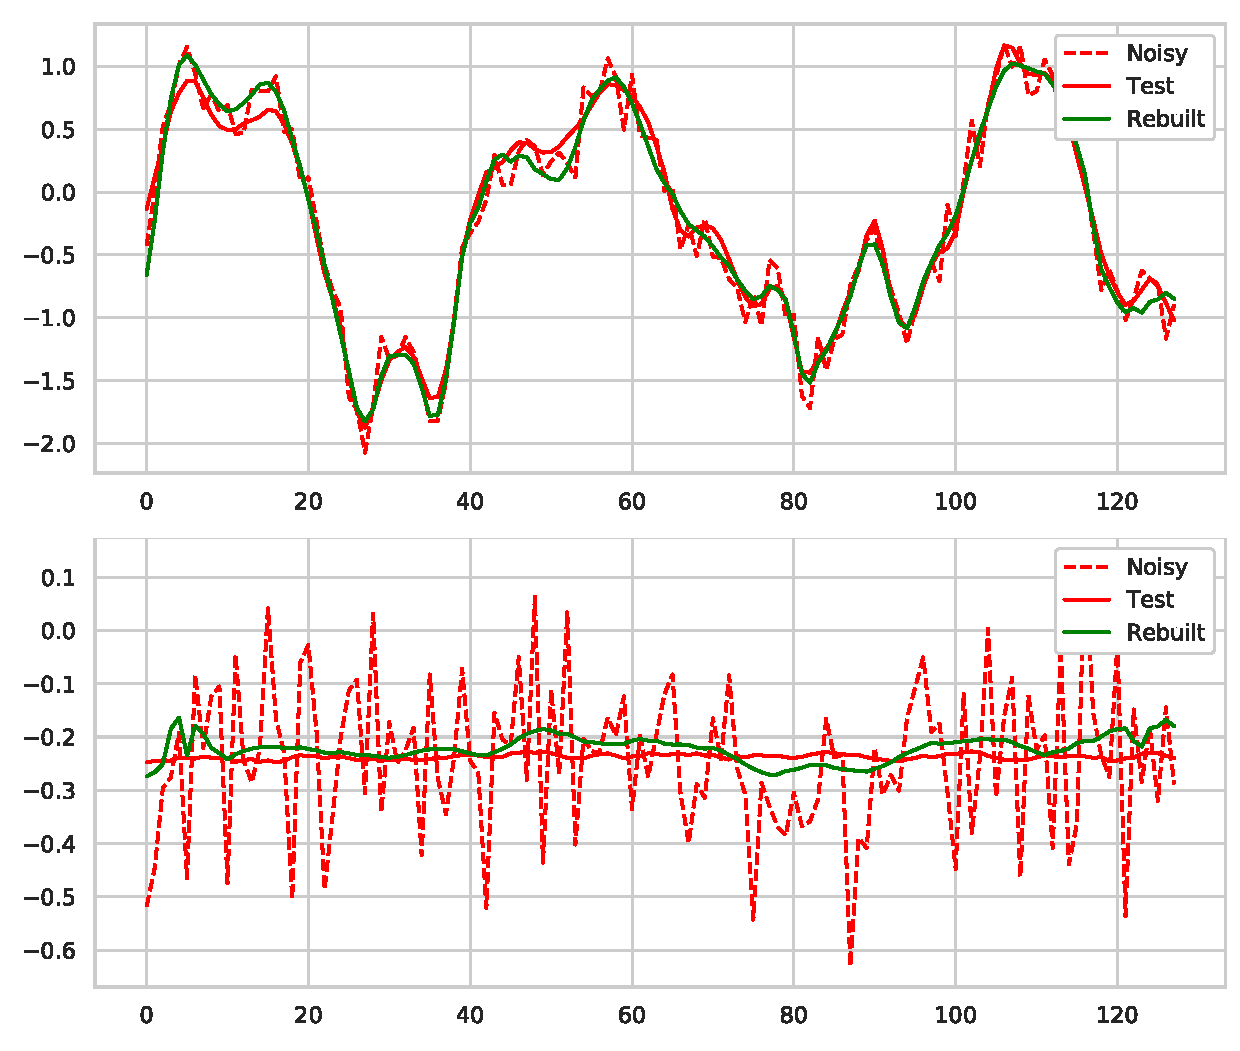
\includegraphics[width=\columnwidth]{ae-signals}
    \caption{Reconstruction of some sample signals done by the first autoencoder of the \texttt{ae-long} model. {\it Noisy} is the noisy input used for training, {\it Test} is the original uncorrupted signal, {\it Rebuilt} is the reconstructed signal by the trained autoencoder.}
    \label{fig:img_signal_reconstruction}
\end{figure}

\tab{ae_comparison_table} Compares the different stacked autoencoders \mbox{F1-Scores}.

\begin{table}[!htbp]
\footnotesize
\captionsetup{font=scriptsize, justification=centering}
\centering
\resizebox{\columnwidth}{!}{%
\begin{tabular}{|r|c|c|c|c|}
\hline
\multicolumn{1}{|c|}{} & \textbf{ae-long-gaus} & \textbf{ae-long-zero} & \textbf{ae-short-gaus} & \textbf{ae-short-zero} \\ \hline
\textbf{Falling} & 0.667 & 0.571 & \textbf{0.720} & 0.656 \\ \hline
\textbf{Jumping} & 0.838 & 0.805 & \textbf{0.849} & 0.766 \\ \hline
\textbf{Lying} & \textbf{0.985} & 0.985 & 0.985 & 0.985 \\ \hline
\textbf{Running} & \textbf{0.956} & 0.945 & 0.947 & 0.949 \\ \hline
\textbf{Sitting} & \textbf{0.867} & 0.823 & 0.850 & 0.847 \\ \hline
\textbf{Standing} & \textbf{0.935} & 0.912 & 0.926 & 0.920 \\ \hline
\textbf{Walking} & \textbf{0.979} & 0.965 & 0.972 & 0.975 \\ \hline
\rowcolor[HTML]{E1E1E1} 
\textbf{Mean} & \textbf{0.934} & 0.911 & 0.925 & 0.921 \\ \hline
\end{tabular}%
}
\caption{F1-Scores for various stacked autoencoders, \texttt{long} prefix indicates the deeper version of the first autoencoder, as presented in \secref{sec:m_ae}, \texttt{short} prefix indicates the shallower version. \texttt{gaus} suffix indicates the model trained with inputs corrupted by gaussian noise, \texttt{zero} instead indicates zero-masking corruption.}
\label{ae_comparison_table}
\end{table}

While the best \mbox{F1-Score} is achieved by \texttt{long-gaus} model with a value of 0.934, with just a 0.009 improvement with respect to the shallower version, the latter was able to achieve a better classification accuracy on underrepresented classes. The deeper version was probably able to build a more complex representation of the input data for classes with a higher number of samples, thus offering an improved \mbox{F1-Score} on specific classes i.e. {\it running, sitting, standing, walking}. Lastly, the autoencoder with gaussian noise performed slightly better compared to the zero-masking one.

\subsection{Overall model comparison}
\label{sec:final_results}
The previous two sections were aimed to find the best version of the analysed models in order to perform additional fine tunings and thus do a final comparison with the remaining model, which is presented in this section.\\
In this section two more models are introduced:
\begin{itemize}
\item \texttt{m_1d2d_01_reg} which has the same topology as \texttt{m_1d2d_01} but adds L2 regularization in the last 2 dense layers
\item \texttt{m_resnet} which is {\it ResNet-50}
\end{itemize}

The models were compared using the \texttt{aug} dataset and the \mbox{F1-scores} are summarized in \tab{final_models_table}.

\begin{table}[!htbp]
\captionsetup{font=scriptsize, justification=centering}
\centering
\resizebox{\columnwidth}{!}{%
\begin{tabular}{r|c|c|c|c|c|c|c|}
\cline{2-8}
 & \textbf{ae-long-gaus} & \textbf{m\_2d} & \textbf{m\_1d2d\_01} & \textbf{m\_1d2d\_01\_reg} & \textbf{m\_1d2d} & \textbf{m\_1d} & \textbf{m\_resnet} \\ \hline
\multicolumn{1}{|r|}{Falling} & 0.667 & 0.838 & 0.879 & \textbf{0.919} & 0.882 & 0.773 & 0.872 \\ \hline
\multicolumn{1}{|r|}{Jumping} & 0.838 & 0.926 & 0.952 & \textbf{0.964} & 0.94 & 0.934 & 0.936 \\ \hline
\multicolumn{1}{|r|}{Lying} & 0.985 & 0.991 & 0.992 & \textbf{0.993} & 0.976 & 0.989 & 0.992 \\ \hline
\multicolumn{1}{|r|}{Running} & 0.956 & 0.991 & 0.998 & \textbf{0.998} & 0.995 & 0.981 & 0.989 \\ \hline
\multicolumn{1}{|r|}{Sitting} & 0.867 & 0.903 & 0.929 & \textbf{0.94} & 0.874 & 0.836 & 0.92 \\ \hline
\multicolumn{1}{|r|}{Standing} & 0.935 & 0.952 & 0.964 & \textbf{0.969} & 0.942 & 0.928 & 0.956 \\ \hline
\multicolumn{1}{|r|}{Walking} & 0.979 & 0.989 & 0.992 & \textbf{0.992} & 0.989 & 0.987 & 0.99 \\ \hline
\rowcolor[HTML]{D9D9D9} 
\multicolumn{1}{|r|}{\cellcolor[HTML]{D9D9D9}Mean} & 0.934 & 0.955 & 0.967 & \textbf{0.972} & 0.945 & 0.932 & 0.961 \\ \hline
\end{tabular}%
}
\caption{F1-Scores of selected models.}
\label{final_models_table}
\end{table}

Training curves of the experiments are depicted in \fig{fig:img_f1_scores}

\begin{figure}[h]
	\captionsetup{font=scriptsize, justification=centering}
    \centering
	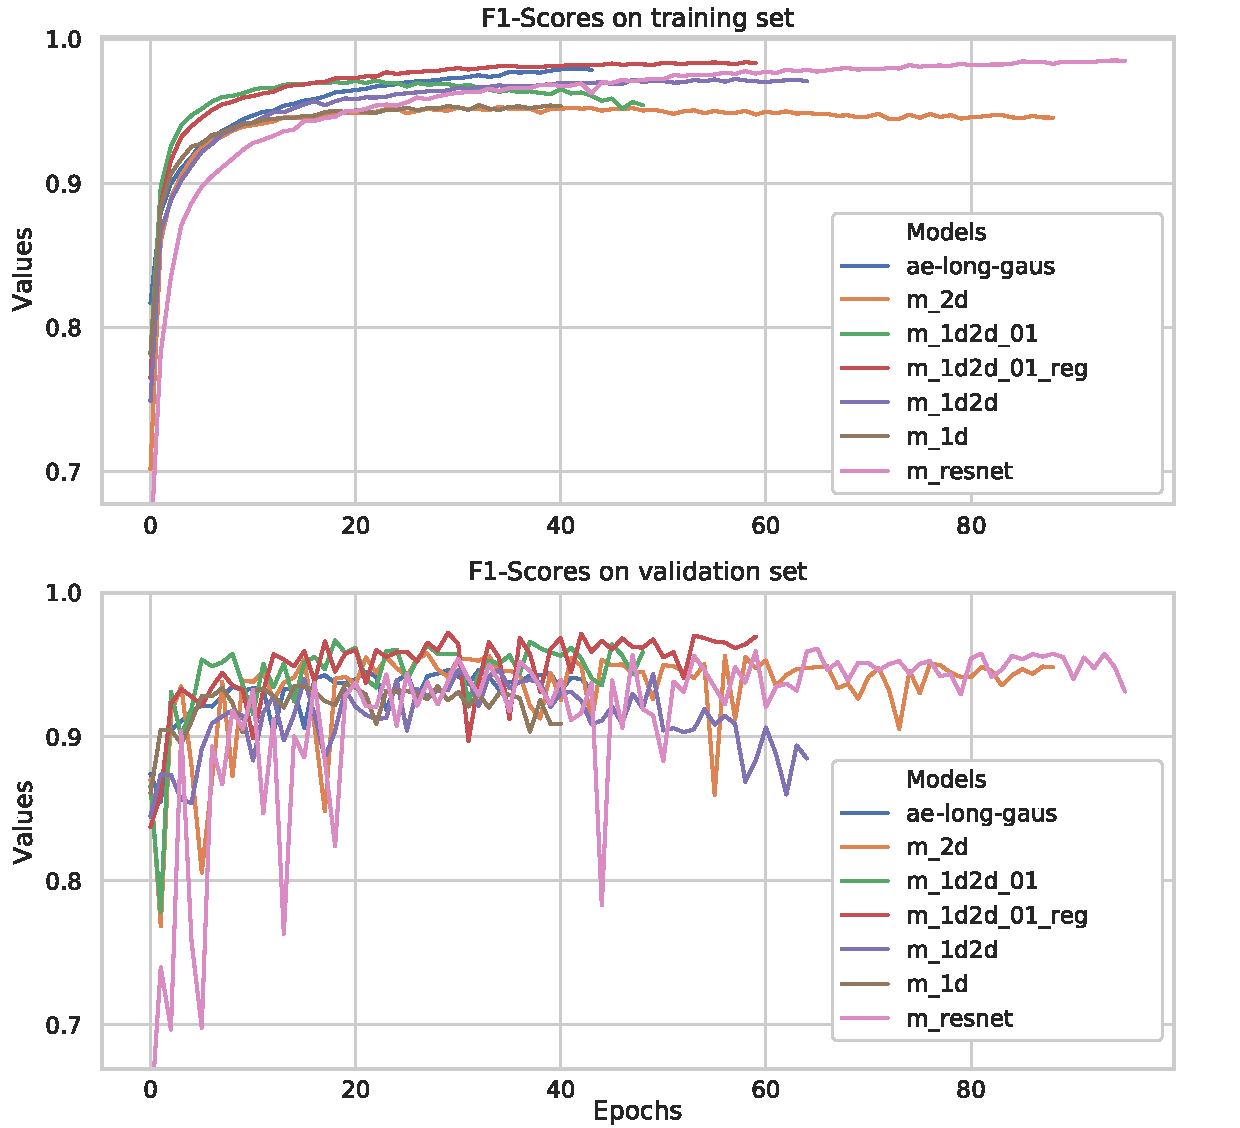
\includegraphics[width=\columnwidth]{f1-scores}
    \caption{F1-Scores for training and validation set.}
    \label{fig:img_f1_scores}
\end{figure}

The regularized version of model \texttt{m_1d2d_01} was able to remove the overfitting problem which is noticeable at approximately 20 epochs (\fig{fig:img_f1_scores}) and thus improves its classification accuracy. Batch size and the learning rate may be influencing the fluctuations in the validation accuracy plot of \fig{fig:img_f1_scores}.\\
Overall the best model achieves an \mbox{F1-Score} of 0.972 and the confusion matrix related to this model is presented in \tab{conf_matrix}

\begin{table}[!htbp]
\captionsetup{font=scriptsize, justification=centering}
\centering
\resizebox{\columnwidth}{!}{%
\begin{tabular}{cc|c|c|c|c|c|c|c|c|}
\cline{3-10}
 &  & \multicolumn{7}{c|}{\cellcolor[HTML]{B2B2B2}\textbf{Predicted}} & \cellcolor[HTML]{E5DFDF} \\ \cline{3-9}
 &  & Falling & Jumping & Lying & Running & Sitting & Standing & Walking & \multirow{-2}{*}{\cellcolor[HTML]{E5DFDF}\textbf{Recall}} \\ \hline
\multicolumn{1}{|c|}{\cellcolor[HTML]{B2B2B2}} & Falling & \textbf{0.92} & 0 & 0.027 & 0 & 0.054 & 0 & 0 & 0.919 \\ \cline{2-10} 
\multicolumn{1}{|c|}{\cellcolor[HTML]{B2B2B2}} & Jumping & 0 & \textbf{0.93} & 0 & 0.007 & 0 & 0.021 & 0.042 & 0.930 \\ \cline{2-10} 
\multicolumn{1}{|c|}{\cellcolor[HTML]{B2B2B2}} & Lying & 0.0057 & 0 & \textbf{0.99} & 0 & 0.0057 & 0 & 0 & 0.989 \\ \cline{2-10} 
\multicolumn{1}{|c|}{\cellcolor[HTML]{B2B2B2}} & Running & 0 & 0 & 0 & \textbf{1} & 0 & 0 & 0 & 1 \\ \cline{2-10} 
\multicolumn{1}{|c|}{\cellcolor[HTML]{B2B2B2}} & Sitting & 0 & 0 & 0 & 0 & \textbf{0.92} & 0.083 & 0 & 0.917 \\ \cline{2-10} 
\multicolumn{1}{|c|}{\cellcolor[HTML]{B2B2B2}} & Standing & 0 & 0 & 0 & 0 & 0.015 & \textbf{0.98} & 0.0013 & 0.984 \\ \cline{2-10} 
\multicolumn{1}{|c|}{\multirow{-7}{*}{\cellcolor[HTML]{B2B2B2}\textbf{True}}} & Walking & 0 & 0 & 0 & 0 & 0 & 0.0096 & \textbf{0.99} & 0.990 \\ \hline
\multicolumn{2}{|c|}{\cellcolor[HTML]{E5DFDF}\textbf{Precision}} & 0.919 & 1 & 0.998 & 0.996 & 0.964 & 0.954 & 0.993 & \textbf{0.972} \\ \hline
\end{tabular}%
}
\caption{Confusion matrix of model \texttt{m_1d2d_01_reg} referred to the \texttt{aug} dataset}
\label{conf_matrix}
\end{table}

As a comparison with the reference paper \cite{base-paper}, \tab{comparison_table} reports the \mbox{F1-Scores} for the best model of this paper and the best model of \cite{base-paper}

\begin{table}[!htbp]
\footnotesize
\captionsetup{font=scriptsize, justification=centering}
\centering
\begin{tabular}{r|c|c|c|}
\cline{2-4}
\multicolumn{1}{c|}{} & \textbf{Reference} & \textbf{m\_1d2d\_01\_aug} & \textbf{Diff} \\ \hline
\multicolumn{1}{|r|}{\textbf{Falling}} & 0.889 & 0.919 & \cellcolor[HTML]{9AFF99}0.03 \\ \hline
\multicolumn{1}{|r|}{\textbf{Jumping}} & 0.930 & 0.964 & \cellcolor[HTML]{9AFF99}0.034 \\ \hline
\multicolumn{1}{|r|}{\textbf{Lying}} & 0.989 & 0.993 & \cellcolor[HTML]{9AFF99}0.004 \\ \hline
\multicolumn{1}{|r|}{\textbf{Running}} & 0.963 & 0.998 & \cellcolor[HTML]{9AFF99}0.035 \\ \hline
\multicolumn{1}{|r|}{\textbf{Sitting}} & 0.984 & 0.940 & \cellcolor[HTML]{FFCE93}-0.044 \\ \hline
\multicolumn{1}{|r|}{\textbf{Standing}} & 0.989 & 0.969 & \cellcolor[HTML]{FFCE93}-0.02 \\ \hline
\multicolumn{1}{|r|}{\textbf{Walking}} & 0.989 & 0.992 & \cellcolor[HTML]{9AFF99}0.003 \\ \hline
\end{tabular}
\caption{F1-Scores of best model of reference paper \cite{base-paper} vs the best model of this paper along with the difference between the two approaches.}
\label{comparison_table}
\end{table}